\chapter{The Fundamental Group $\pi_1(M)$} \thispagestyle{empty}

In the previous chapter, we proved that the Lie algebra $\mathrm{so}(3, \, \R)$ is isomorphic to the Lie algebra $\mathrm{su}(2, \, \C)$, as they have the same universal constants.

The goal of this chapter is to introduce a powerful mathematical tool, called \textit{fundamental group}\index{fundamental group}, which will allow us to answer the question
\begin{equation*} \mathrm{SO}(3) \stackrel{?}{\cong} \mathrm{SU}(2). \end{equation*}
Furthermore, we shall explore the connection between the local behavior and the global behavior of these two groups employing the notion of \textit{covering space}\index{covering space}.

\section{Homotopy}

In this chapter, we develop the homotopy theory for a topological space\index{topological space} $M$ (i.e., a space equipped with a topology $\tau$), but the reader with no topology background may think of $M$ as a manifold.

In topology, there is a somewhat intuitive notion that measures, in a certain sense, how similar two (geometrical) objects are.

For example, the union between the circumference $S^1$ and its diameter is intuitively equivalent to the union of two tangent $S^1$. We shall soon be able to give a precise meaning to this statement, and we will also be able to prove it formally.

\begin{figure}[h]
        \centering{ \scalebox{.7}{ 
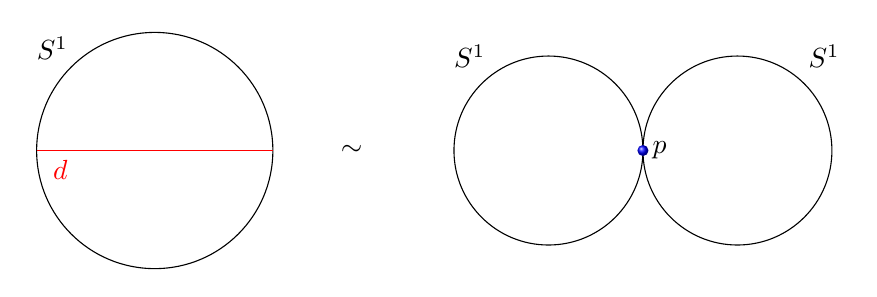
\begin{tikzpicture}
	\draw (0,0) circle (1.5cm);
	\node (A) at (-1.3, 1.3) {$S^1$};
	\draw[-,ultra thin, red] (-1.5,0)--(1.5,0) node[pos =0.1, below]{$d$};
	\node (B) at (2.5, 0) {$\sim$};
	\draw (5,0) circle (1.2cm);
	\draw (7.4,0) circle (1.2cm);
	\node (B) at (4, 1.2) {$S^1$};
	\node (C) at (8.5, 1.2) {$S^1$};
		[anchor=mid west,
			mark size=+2pt, mark color=red,  ball color=green]
			\foreach \plm[count=\cnt] in {ball}
			\draw[mark options={fill=red}]
			plot[mark=\plm] coordinates {(6.2, 0)} node[right]{$p$};
\end{tikzpicture}
}
	\caption{The union of a circumference with its diameter $S^1 \cup d$ is equivalent to the union $S^1 \cup S^1$ between tangent circumferences.}
	}
\end{figure}

\vspace{1cm}

\subsection{Path-Components}

The goal of this section is to introduce the $\pi_0(M)$, which is the set of all the path-connected components\index{path-connected components} of $M$. We first need to recall some basic topological notions (e.g., connectedness, path-connectedness, connected components, etc.)

\begin{definition}\index{connected set}\index{connectedness} A topological space $M$ is \textit{disconnected} if there are two nonempty proper open sets $A, \, B \subset M$ such that $A \cup B = M$. A topological space is \textit{connected} if it is not disconnected. \end{definition}

\vspace{1cm}

\begin{figure}[h]
        \centering{
        \scalebox{.8}{
\begin{tikzpicture}
	\draw (0,0) circle (1.5cm);
	\node (A) at (-1.3, 1.3) {$S^1$};
	\draw (5,0) circle (1.2cm);
	\draw (8,0) circle (1.2cm);
	\node (B) at (4, 1.2) {$S^1$};
	\node (C) at (9, 1.2) {$S^1$};
\end{tikzpicture}}
	\caption{The circumference $S^1$ is connected and path-connected, while the disjoint union $S^1 \sqcup S^1$ is disconnected and has two connected components.}
	}
\end{figure}

\vspace{1cm}

\begin{definition}\index{path-connected set}\index{path-connectedness} A topological space $M$ is \textit{path-connected} if for every $x, \, y \in M$ there exists a continuous path $\alpha : [0, \, 1] \longrightarrow M$ such that $\alpha(0) = x$ and $\alpha(1) = y$.\end{definition}

\begin{remark}A path-connected topological space $M$ is also connected. \end{remark}

\begin{definition}\index{connected component}Let $M$ be a topological space. A subset $C \subset M$ is a \textit{connected component} of $M$ if the following properties are satisfied: \mbox{}
\begin{enumerate}[label=\textbf{(\arabic*)}]
\item $C$ is connected.
\item $C$ is maximal with respect to the inclusion. Namely, if $C \subseteq A$ and $A$ is connected, then $A = C$.
\end{enumerate} \end{definition}

\begin{definition}[Locally Connected] \index{locally connected}A topological space $M$ is \textit{locally connected} if every point $x \in M$ admits a neighborhood basis made up of connected open sets.  \end{definition}

\begin{remark}A connected topological space $M$ needs not to be a locally connected space. \end{remark}

We are finally ready to introduce the notion of $\pi_0(M)$. Let $M$ be a topological space, and let us consider the equivalence relation defined by
\begin{equation*}x \sim y \iff \text{$\exists \: \alpha : [0, \, 1] \longrightarrow M$ continuous such that $\alpha(0) = x$ and $\alpha(1) = y$}. \end{equation*}
It is an easy exercise to prove that $\sim$ is actually an equivalence relation. The product between two paths can be defined by
\begin{equation*} \alpha \ast \beta(t) := \begin{cases} \alpha(2t) & \text{if $0 \leq t \leq 1/2$}, \\[0.8em] \beta(2t - 1) & \text{if $1/2 \leq t \leq 1$}, \end{cases} \end{equation*}
while the inverse of a path is given by
\begin{equation*} i(\alpha)(t) := \alpha(1 - t). \end{equation*}
The set $\pi_0(M)$ is the set of all the equivalence classes of $M$ with respect to $\sim$. \caution{The set $\pi_0(M)$, in general, \underline{is not a group!}}These equivalence classes are called \textit{path-connected components}\index{path-connected components} of $M$.

\begin{definition}[Locally Path-Connected] \index{locally path-connected}A topological space $M$ is \textit{locally path-connected} if every point $x \in M$ admits a neighborhood basis made up of path-connected open sets.  \end{definition}

In particular, it turns out that two topological spaces (or manifolds/Lie groups) $M$ and $N$ are not homeomorphic if the $\pi_0(\cdot)$'s are different. Unfortunately, both $\mathrm{SO}(3)$ and $\mathrm{SU}(2)$ are path-connected and locally path-connected topological groups, and hence
\begin{equation} \label{eq.4.5} \pi_0( \mathrm{SO}(3) ) = \pi_0 ( \mathrm{SU}(2) ), \end{equation}
which means that we need to introduce a more sophisticated tool to distinguish them, which will turn out to be the fundamental group $\pi_1( \cdot)$.

\subsection{Homotopy}

We now introduce an equivalence relation between continuous maps, called \textit{homotopy}, that will make more precise the meaning of \eqref{eq.4.5}. In the next section, we will refine the notion of homotopy to present the fundamental group finally.

\begin{definition}[Homotopy] \index{homotopic}\index{homotopy} Two continuous maps $f, \, g : M \longrightarrow N$ between topological space are \textit{homotopic} if there exists a continuous map
\begin{equation*} F : M \times [0, \, 1] \longrightarrow N, \end{equation*}
called \textit{homotopy}, such that $F(x, \, 0) = f(x)$ and $F(x, \, 1) = g(x)$ for every $x \in M$. \end{definition}

\begin{example}Two continuous maps $f$ and $g$, defined on a convex set $C \subset \R^n$, are always homotopic. Indeed, it suffices to consider the homotopy
\begin{equation*} F(x, \, t) := (1-t) f(x) + t g(x) \quad \text{for $x \in C$ and $t \in [0, \, 1]$}. \end{equation*} \end{example}

\paragraph{N.B.} The notion of homotopy defines on $C^0(M; \, N)$, the set of all continuous maps between $M$ and $N$, an equivalence relation $\sim$ which is given by
\begin{equation*} f \sim g \iff \text{there exists a continuous homotopy $F$ between $f$ and $g$} \end{equation*}
The formal proof that $\sim$ is actually an equivalence relation is very similar to the one we presented above for paths, and hence we will not write it down here. It is interesting to notice that the homotopy is stable under product (=composition), that is,
\begin{equation*} f_0 \sim f_1 \quad \text{and} \quad g_0 \sim g_1 \implies f_0 \ast g_0 \sim f_1 \ast g_1, \end{equation*}
where $f_0, \, f_1 : M \longrightarrow N$ and $g_0, \, g_1 : N \longrightarrow P$ are continuous mappings between topological spaces.

\begin{definition}[Homotopic Equivalence] \index{homotopic equivalence}A continuous mapping $f : M \longrightarrow N$ between topological spaces is a \textit{homotopic equivalence} if there exists a continuous map $g : N \longrightarrow M$ such that
\begin{equation*} f \circ g \sim \mathrm{id}_N \quad \text{and} \quad g \circ f \sim \mathrm{id}_M. \end{equation*}
Furthermore, two topological space are said to be \textit{homotopic equivalent} if there exists a homotopic equivalence between them. \end{definition}

If $M$ and $N$ are homeomorphic topological spaces (or, in our case, $\G$ and $\G^\prime$ are isomorphic topological groups), then they are also homotopic equivalent.

The fundamental result of this section is the following one. If $f : M \longrightarrow N$ is a homotopic equivalence, then it turns out that $\pi_0(M)$ is isomorphic to $\pi_0(N)$, which means that
\begin{equation*} \pi_0(M) \neq \pi_0(N) \implies \text{$M$ and $N$ are not homotopic equivalent} \implies M \not \cong N, \end{equation*}
and this explains the importance of this notion.

\begin{definition}[Contractible] \index{contractible topological space}A topological space $X$ is \textit{contractible} if it is homotopic equivalent to a point. Equivalently, $X$ is contractible if the identity map $\mathrm{id}_X$ is homotopic to a constant map.\end{definition}

\section{The Fundamental Group}

Let $\alpha : [0, \, 1] \longrightarrow M$ be a closed path (that is, $\alpha(0) = \alpha(1) = x_0$.) In this section, we shall finally refine the notion of homotopy for closed paths of base point $x_0$, and introduce the fundamental group $\pi_1(M, \, x_0)$. 

\subsection{Path Homotopy}

Let $x, \, y \in M$ be two points in a topological space. We define the set of all continuous paths between $x$ and $y$ as follows:
\begin{equation*} \Omega(M, \, x, \, y) := \left\{ \alpha : [0, \, 1] \longrightarrow M \: : \: \text{$\alpha$ is continuous, $\alpha(0) = x$ and $\alpha(1) = y$} \right\}. \end{equation*}

\begin{definition}[Path Homotopy] \index{path homotopic}\index{path homotopy} Two continuous paths $\alpha, \, \beta \in \Omega(M, \, x, \, y)$ are \textit{path homotopic} if there exists a continuous map
\begin{equation*} F : [0, \, 1] \times [0, \, 1] \longrightarrow M, \end{equation*}
called \textit{path homotopy}, such that
\begin{equation*} \begin{aligned} & \text{$F(t, \, 0) = \alpha(t)$ and $F(t, \, 1) = \beta(t)$} \quad \text{for every $t \in [0, \, 1]$}, \\[1em]
& \text{$F(0, \, s) = x$ and $F(1, \, s) = y$} \quad \text{for every $s \in [0, \, 1]$}.\end{aligned} \end{equation*} \end{definition}

The second condition can be easily rewritten as follows. If we let $F_s(\cdot) := F(\cdot, \, s)$, then we are requiring that the continuous path $F_s$ belongs to $\Omega(M, \, x, \, y)$ for every $s \in [0, \, 1]$.

The reader may prove easily that the existence of a path homotopy is also an equivalence relation, denoted by $\sim$, in the set $\Omega(M, \, x, \, y)$. Moreover, both the product of (concatenation) paths and the inverse element commute with the homotopy equivalence relation, which means that
\begin{equation*} \alpha_0 \sim \alpha_1 \quad \text{and} \quad \beta_0 \sim \beta_1 \implies \alpha_0 \ast \beta_0 \sim \alpha_1 \ast \beta_1, \end{equation*}
where $\alpha_i \in \Omega(M, \, x, \, y)$ and $\beta_i \in \Omega(M, \, y, \, z)$, and
\begin{equation*} \alpha_0 \sim \alpha_1 \implies i(\alpha_0) \sim i(\alpha_1). \end{equation*}
The product $\ast$ is associative up to homotopy, that is, given $\alpha \in \Omega(M, \, x, \, y)$, $\beta \in \Omega(M, \, y, \, z)$, and $\gamma \in \Omega(M, \, z, \, w)$, it turns out that
\begin{equation*}(\alpha \ast \beta) \ast \gamma \sim \alpha \ast (\beta \ast \gamma),\end{equation*}
which means that we have the equality as equivalence classes:
\begin{equation*}\left[ (\alpha \ast \beta) \ast \gamma \right] = \left[ \alpha \ast (\beta \ast \gamma) \right]\end{equation*}
In a similar fashion, one can prove that given $\alpha \in \Omega(M, \, x, \, y)$ and $\beta \in \Omega(M, \, x, \, y)$ it turns out that
\begin{equation*} \begin{aligned} & \mathbf{x} \ast \alpha \sim \alpha \ast \mathbf{y} \sim \alpha \implies [\mathbf{x} \ast \alpha] = [\alpha \ast \mathbf{y}] = [\alpha], \\[1em] & \alpha \ast i(\alpha) \sim \mathbf{x}  \implies [\alpha \ast i(\alpha)] = [\mathbf{x}], \end{aligned} \end{equation*}
where $\mathbf{x}$ and $\mathbf{y}$ denote the constant mappings $\mathbf{x}(t) := x$ and $\mathbf{y}(t) := y$ for all $t \in [0, \, 1]$ respectively.

\subsection{The Fundamental Group}

The \textit{fundamental group}\index{fundamental group} of a topological space (or manifold) $M$ with base point $x_0 \in M$ is given by the set of all the equivalence classes $[\alpha]$ for $\alpha \in \Omega(M, \, x_0, \, x_0)$ closed path, and $\sim$ path homotopic equivalence.

\begin{theorem}The set $\pi_1(M, \, x_0)$ endowed with the path product $\ast$ is a group, where the identity element is the path $\mathbf{x_0}$, and the inverse element is given by $i(\cdot)$. \end{theorem}

The group $\pi_1(M, \, x_0)$ does not depend on $x_0$ as an individual point, but rather on the entire path-connected component containing $x_0$. Hence, if $M$ is a path-connected space
\begin{equation*} \pi_1(M, \, x_0) \cong \pi_1(M, \, y_0) \quad \text{for every $x_0, \, y_0 \in M$}, \end{equation*}
and thus we can drop the notation $\pi_1(M, \, x_0)$ and simply write $\pi_1(M)$.

Since both $\mathrm{SO}(3)$ and $\mathrm{SU}(2)$ are path-connected, this simple remark will be extremely useful in the last part of this chapter.

\begin{definition}[Simply Connected]\index{simply connected space}A topological space $M$ is \textit{simply connected} if $M$ is path-connected and $\pi_1(M) = \{e\}$ is the trivial group. \end{definition}

\subsection{Examples}

We will develop more the theory of the fundamental group in the next section after we have introduced the notion of \textit{covering space}. Here we present some examples of $\pi_1(-)$ that can be computed explicitly with some efforts.

\begin{theorem}The fundamental group of $S^1$ is isomorphic to $\Z$. \end{theorem}

\begin{proof}This result is highly nontrivial, and a proof can be found in \cite[pp. 29--32]{hatcher}. \end{proof}

\begin{theorem}\label{thm.sc1} The fundamental group of $S^n$ is trivial for every $n \geq 2$. \end{theorem}

\begin{proof}This assertion follows from a straightforward application of the Van Kampen's theorem. The interested reader may consult \cite[pp. 43--52]{hatcher} for a more detailed discussion. \end{proof}

\begin{theorem}The fundamental group of the torus $\T$ is isomorphic to $\Z \times \Z$. \end{theorem}

\begin{proof}The torus $\T$ is isomorphic to $S^1 \times S^1$, and therefore it is enough to show that
\begin{equation*} \pi_1(M \times N) \cong \pi_1(M) \times \pi_1(N) \end{equation*}
for path-connected topological spaces $M$ and $N$.\end{proof}

\begin{theorem}Let $M$ be a contractible manifold (or topological space). Then the fundamental group of $M$ is trivial. \end{theorem}

Before we can talk about our last, fundamental, example, we need to briefly introduce the $n$-dimensional real projective space\footnote{The projective space is a smooth manifold, i.e. a manifold of class $C^\infty$.} $\R \p^n$. We consider the equivalence relation
\begin{equation*} x \sim_\imath y \iff \exists \: \lambda \in \R \setminus \{0\} \: : \: x = \lambda y, \end{equation*}
and we define the real projective space as the quotient
\begin{equation*} \R \p^n := \faktor{\R^{n + 1} \setminus \{0\} }{\sim_\imath}. \end{equation*}
Intuitively, the projective space is the set of all the lines through the origin in $\R^{n + 1}$, and therefore one can easily prove that we also have
\begin{equation*} \R \p^n := \faktor{S^n }{\sim_\imath}, \end{equation*}
where $S^n := \left\{x \in \R^{n + 1} \: : \: |x| = 1 \right\}$ and $x \sim_\imath y$ if and only if $x = - y$.

\begin{theorem} \label{thm.sc2} The fundamental group of the real projective space $\R \p^n$ is isomorphic to $\Z_2$ (=$\mathcal{C}_2$) for every $n \geq 2$. \end{theorem}

\begin{proof}The reader may consult \cite[pp. 71--73]{hatcher}.  \end{proof}

\section{Covering Space}

\begin{definition}[Covering Space] \index{covering space} A \textit{topological covering} is a continuous surjective map of topological spaces
\begin{equation*} p : \widetilde{M} \longrightarrow M \end{equation*}
 such that, for every $x \in M$, there exists an open neighborhood $U_x \subset M$ of $x$, such that
\begin{equation*} p^{-1} (U_x) = \bigsqcup_{i \in \mathcal{I}} U_i, \end{equation*}
where $\{U_i\}_{i \in \mathcal{I}}$ is a disjoint collection (eventually infinite) of open sets $U_i \subset \widetilde{M}$ such that
\begin{equation*} p \, \big|_{U_i} : U_i \longrightarrow U_x \end{equation*}
is a homeomorphism\footnote{A homeomorphism $f : X \longrightarrow Y$ is an invertible continuous map between topological spaces such that $f^{-1} : Y \longrightarrow X$ is also continuous. } for every $i \in \mathcal{I}$.  \end{definition}

The space $\widetilde{M}$ is called \textit{total space}, the space $M$ is the \textit{base space}, and the sets $p^{-1}(x)$ are the \textit{fibers} of the covering $p$.

\begin{definition}[Degree] \index{covering space!degree} If every fiber of $p : \widetilde{M} \longrightarrow M$ is finite and of cardinality $d$, we say that $p$ is a covering of degree $d$. If the cardinality is infinite, we simply say that $p$ is a covering of infinite ($\infty$) degree. \end{definition}

\begin{example}[Circle] The (universal) covering of $S^1$ is given by
\begin{equation*}\R \ni t \longmapsto \mathrm{e}^{2 \pi \imath \cdot t} \in S^1, \end{equation*}
and it degree is equal to infinity.  \end{example}

\begin{example}[Complex Polynomial] The map
\begin{equation*}\C \setminus \{0\} \ni z \longmapsto z^n \in \C \setminus \{0\}, \end{equation*}
is a covering of degree $n$ for every $n \geq 1$.  \end{example}

\begin{example}[Projective Space] \label{ex.4.1} Let $n \geq 2$. The natural projection
\begin{equation*}\pi : S^n \longrightarrow \faktor{S^n}{\sim_\imath} = \R \p^n\end{equation*}
that sends a point $x$ to its equivalence class $[x] := \{x, \, -x\}$ is a covering of degree two. \end{example}

\section{Application: $\mathrm{SU}(2, \, \C) \not \cong \mathrm{SO}(3, \, \R)$}

In this final section, the goal is to prove that $\mathrm{SU}(2, \, \C)$ is isomorphic to the sphere $S^3$ and $\mathrm{SO}(3, \, \R)$ is isomorphic to the real projective space $\R \p^3$. From \hyperref[thm.sc1]{Theorem \ref{thm.sc1}} and \hyperref[thm.sc2]{Theorem \ref{thm.sc2}} it will follow easily that
\begin{equation*} \pi_1 \left( \mathrm{SU}(2, \, \C) \right) = \{e\} \neq \Z_2 \cong \pi_1 \left( \mathrm{SO}(3, \, \R) \right), \end{equation*}
and thus $\mathrm{SU}(2, \, \C) \not \cong \mathrm{SO}(3, \, \R)$. Moreover, we will also be able to find a covering
\begin{equation*}\pi : \mathrm{SU}(2, \, \C) \longrightarrow\mathrm{SO}(3, \, \R) \end{equation*}
of degree $2$, that is, a surjective map between the two groups which is also $2$-to-$1$.

We will not give an entirely formal proof of the following results, but we will only describe the main ideas behind them and leave it to the reader to fill in the details.

\begin{theorem}The special orthogonal group $\mathrm{SO}(3, \, \R)$ is isomorphic to $\R \p^3$. \end{theorem} \caution[b][darkgreen][Note]{Actually, the same proof shows that $\mathrm{SO}(3, \, \R)$ is diffeomorphic to $\R \p^3$.}

\begin{proof} The group $\mathrm{SO}(3, \, \R)$ consists in all the rotations of $\R^3$, and these are characterized uniquely by the choice of an oriented vector $\vec{v} \in S^2$ and an angle $\theta \in [0, \, 2\pi)$. If we denote by $R(\vec{v}, \,\theta)$ a rotation, it is easy to prove that
\begin{equation*} R(\vec{v}, \, \pi) = R(- \vec{v}, \, \pi) \quad \text{and} \quad R(\vec{v}, \, 0) = R(\vec{w}, \, 0), \end{equation*}
which means that we can define a mapping
\begin{equation*} \varphi : \mathrm{SO}(3, \, \R) \longrightarrow \faktor{S^3}{\sim_\imath} \end{equation*}
that sends $R(\vec{v}, \, \theta)$ to the equivalence class $[v \cdot \theta]$. The reader can easily prove using the definition that $\varphi$ is continuous, bijective, and its inverse $\varphi^{-1}$ is also continuous. \end{proof}

\begin{theorem}\label{thm.5.2} The special unitary group $\mathrm{SU}(2, \, \C)$ is isomorphic to $S^3$. \end{theorem}
\caution[b][darkgreen][Note]{Actually, the same proof shows that $\mathrm{SU}(2, \, \C)$ is diffeomorphic to $S^3$.}

\begin{proof} The $3$-sphere $S^3$ in $\R^4$ can be identified with the complex sphere
\begin{equation*} S_\C^1 := \left\{ (z, \, w) \in \C^2 \: : \: |z|^2 + |w|^2 = 1 \right\}, \end{equation*}
and thus it suffices to prove that $S_\C^1 \cong \mathrm{SU}(2, \, \C)$. On the other hand, one can easily check that
\begin{equation} \label{eq.4.100} U \in \mathrm{SU}(2) \implies U = \begin{pmatrix}z & - \bar{w} \\ w & \bar{z} \end{pmatrix} \quad \text{and} \quad \mathrm{det}(U) = |z|^2 +|w|^2 = 1. \end{equation}
If we identify the unitary matrix \eqref{eq.4.100} with the symbol $U_{z,  \,w}$, then we can easily define a mapping
\begin{equation*} \psi : \mathrm{SU}(2, \, \C) \longrightarrow S_\C^1 \end{equation*}
that sends $U_{z, \, w}$ to $(z, \, w) \in \C^2$. Clearly, $\psi$ is invertible and its inverse is given by
\begin{equation*} \psi^{-1} : S_\C^1 \ni (z, \, w) \longmapsto \begin{pmatrix}z & - \bar{w} \\ w & \bar{z} \end{pmatrix} \in \mathrm{SU}(2, \, \C), \end{equation*}
and, as the reader may check by herself, both are continuous.\end{proof}

\section{Monodromy Group}

Let $p : M\longrightarrow N$ be a covering, and let $x, \, y \in N$ be any two points in the base space. The \textit{monodromy}\index{monodromy mapping} mapping associated to $p$ is given by
\begin{equation*}\mathrm{Mon} : p^{-1}(x) \times \Omega(N, \, x, \, y) \longrightarrow p^{-1}(y), \qquad \mathrm{Mon}(e, \, \alpha) := \alpha_e(1), \end{equation*}
where $\alpha_e : I \longrightarrow M$ is the unique path lifting\index{path lifting}\footnote{Let $p : M \longrightarrow N$ be a covering and $\alpha : I \longrightarrow N$ a path. A path $\gamma : I \longrightarrow M$ is a lifting of $\alpha$ if and only if the diagram is commutative, that is $p \circ \gamma = \alpha$.} of $\alpha$ such that $\alpha_e(0) = e$. For any path $\beta \in \Omega(N, \, y, \, z)$ it is easy to prove that
\begin{equation*}(\alpha \ast \beta)_e = \alpha_e \ast \beta_{\alpha_e(1)}, \end{equation*}
where $\ast$ is the path multiplication. It follows that
\begin{equation} \label{eq.5.1} \mathrm{Mon}(e, \, \alpha \ast \beta) = \mathrm{Mon} \left( \mathrm{Mon}(e, \, \alpha), \, \beta \right). \end{equation}
We will not prove it here, but the monodromy $\mathrm{Mon}(e, \, \alpha)$ depends only on the homotopy class of the path $\alpha$, and hence
\begin{equation*} \mathrm{Mon} \left(e, \, \alpha \ast i(\alpha) \right) = \mathrm{Mon}(e, \, \mathbf{x}) = e. \end{equation*}
It follows that for any $\alpha \in \Omega(N, \, x, \, y)$, the mappings
\begin{equation*}p^{-1}(x) \longrightarrow p^{-1}(y), \qquad e \longmapsto \mathrm{Mon}(e, \, \alpha) \end{equation*}
is bijective, whose inverse is given by
\begin{equation*}p^{-1}(y) \longrightarrow p^{-1}(x), \qquad e \longmapsto \mathrm{Mon}(e, \, i(\alpha)) \end{equation*}
If $x = y$, then the monodromy mapping associated to $p$ acts on the $\pi_1(N, \, x)$, that is,
\begin{equation*}\mathrm{Mon} : p^{-1}(x) \times \pi_1(N, \, x) \longrightarrow p^{-1}(y), \qquad \mathrm{Mon}(e, \, [\alpha]) := \alpha_e(1), \end{equation*}
where $[\alpha]$ denotes the equivalence class of $\alpha$. The monodromy mapping sends the constant path $\mathbf{x}$ to the identity element in $p^{-1}(x)$, and similarly from \eqref{eq.5.1} we infer that
\begin{equation*}\mathrm{Mon}(e, \, [\alpha \ast \beta]) = \mathrm{Mon} \left( \alpha_e(1), \, [\beta] \right) = \beta_{\alpha_e(1)}(1). \end{equation*}
More intuitively, the monodromy map permutes the points in the fiber $p^{-1}(x) = \{ a_j \}_{j \in \mathcal{J}}$. In fact, given a closed loop $[\alpha] \in \pi_1(N, \, x)$, the lifting $\alpha_{a_j}$, for some $j \in \mathcal{J}$, does not necessarily satisfies $\alpha_{a_j}(1) = a_j$, but it could happen that $\alpha_{a_j}(1) = a_k$ for a $k \in \mathcal{J}$ different from $j$.

In particular, we associate a permutation matrix $\sigma(\alpha)$, called \textit{monodromy matrix}\index{monodromy matrix}, to the path $\alpha$ in such a way that
\begin{equation*} \begin{pmatrix} a_1 \\ a_2 \\ \vdots \end{pmatrix} \xrightarrow{\alpha_{a_j}}\begin{pmatrix} a_{\sigma(1)} \\ a_{\sigma(2)} \\ \vdots \end{pmatrix} = \begin{pmatrix} & & \\ & \sigma(\alpha) & \\ & & \end{pmatrix} \begin{pmatrix} a_1 \\ a_2 \\ \vdots \end{pmatrix}. \end{equation*}
The square matrix $\sigma(\alpha)$ has a number of row/column equal to the grade of the covering $p$, which means that it could be infinite-dimensional. The monodromy matrix depends only on the homotopy class of $\alpha$, and we also have that
\begin{equation*} \sigma( \alpha \ast \beta ) = \sigma(\alpha) \sigma(\beta) \end{equation*}
as a consequence of \eqref{eq.5.1}. It follows that
\begin{equation*} \left\{ \sigma(\alpha) \: \left| \: [\alpha] \in \pi_1(N, \, x) \right. \right\} \end{equation*}
is a matrices group, which gives us a representation of the fundamental group $\pi_1(N, \, x)$. We denote it by $\sigma(\pi_1(N, \, x))$, and we call it \textit{monodromy group}\index{monodromy group}.

\subsection{Examples}

In this section, we investigate some simple examples of covering spaces, and we compute the respective monodromy groups.

\begin{example}[Circle] Recall that the (universal) covering of $S^1$ is given by
\begin{equation*}\R \ni t \longmapsto \mathrm{e}^{2 \pi \imath \cdot t} \in S^1, \end{equation*}
and the fundamental group of $S^1$ is isomorphic to $\Z$. The integer $m \in \Z$ corresponding to a closed loop $[\alpha] \in \pi_1(S^1)$ is, intuitively, equal to the "number of laps", which means that the monodromy matrix is simply given by a translation
\begin{equation*} \sigma(m) : x \longmapsto x + m \quad \text{for $m \in \Z \cong \pi_1(S^1)$}.\end{equation*} 
Therefore, the monodromy group is the additive group of integer translation, i.e. $\sigma(\pi_1(S^1)) \cong \Z$ once again.\end{example}

\begin{example}We consider the covering of degree $n$
\begin{equation*}\C \setminus \{0\} \ni z \longmapsto z^n \in \C \setminus \{0\}, \end{equation*}
and we identify $\C \setminus \{0\}$ with $S^1$ in the usual way. The fundamental group of $S^1$ is still $\Z$, but in this case the monodromy matrix is slightly different since an entire "lap" ($m = 1$) corresponds to a rotation of $2 \pi/n$ of the $n$th roots of the unity. Namely, we have
\begin{equation*}\sigma(1) = \begin{pmatrix} 0 & \dots & 0 & 1 \\ 1 & \dots & 0 & 0 \\ \vdots & \ddots & \vdots& \vdots \\ 0 & \dots & 1 & 0 \end{pmatrix}, \quad \dots, \quad  \sigma(n-1) = \begin{pmatrix} 0 & 1 & \dots & 0  \\ \vdots & \vdots & \ddots& \vdots \\ 0 & 0 & \dots & 1 \\1 & 0 & \dots & 0  \end{pmatrix},\end{equation*} 
and it is easy to prove that $\sigma(i + n) = \sigma(i)$ for every $i \in \{0, \, \dots, \, n-1\}$. In particular, the monodromy group $\sigma(\pi_1(S^1))$ is isomorphic to the cyclic group $\Z_n$ (=$\mathcal{C}_n$).\end{example}

\begin{example}Let $n \geq 2$. We notice in the previous sections that the natural projection
\begin{equation*}\pi : S^n \longrightarrow \faktor{S^n}{\sim_\imath} = \R \p^n\end{equation*}
that sends a point $x$ to its equivalence class $[x] := \{x, \, -x\}$ is a covering of degree two. The fundamental group of $\R \p^n$ is isomorphic to $\Z_2$, which means that the monodromy group consist in only two elements:
\begin{equation*} \sigma(0)(x) = x \quad \text{and} \quad \sigma(1)( \pm x) = \mp x. \end{equation*}
In particular, the monodromy group $\sigma(\pi_1(\R \p^n))$ is also isomorphic to $\Z_2$. \end{example}

\section{Higher-Order Homotopy Groups}

Homotopy theory begins with the notion of generalized homotopy group $\pi_n(M)$ for $n \geq 2$. These allow us to "distinguish", in a certain sense, the class of homeomorphism of topological spaces (i.e., Lie groups) as follows. If $M$ and $N$ are two topological groups such that
\begin{equation*} \exists \, i \geq 0 \: : \: \pi_i(M) \not \cong \pi_i(N), \end{equation*}
then one can infer that $M \not \cong N$. Unfortunately, the opposite assertion
\begin{equation*}  \pi_i(M) \cong \pi_i(N) \quad \text{for all $i \geq 0$} \implies M \cong N \end{equation*}
is false, as one can easily check by taking $M := \R$ and $N = \{x_0\}$. Furthermore, the higher-order homotopy groups are usually hard to compute than the fundamental group, due to the fact that the Van Kampen's theorem does not hold for $\pi_n$, $n \geq 2$.

Before we give the formal definition of $\pi_n(M)$ for any $n \geq 2$, we take a look at some of the computations of the group $\pi_i(S^n)$ presented in \cite{toda}.

\begin{figure}[h!]
\begin{flushleft}
\begin{tikzpicture}
\clip node (m) [matrix,matrix of nodes,
fill=black!20,inner sep=0pt,
nodes in empty cells,
nodes={minimum height=1cm,minimum width=1cm,anchor=center,outer sep=0,font=\sffamily},
row 1/.style={nodes={fill=black,text=white}},
column 1/.style={nodes={fill=gray,text=white,align=center,text width=1.5cm,text depth=0.5ex}},
column 2/.style={text width=0.5cm,align=center,every even row/.style={nodes={fill=white}}},
column 3/.style={text width=0.5cm,align=center,every even row/.style={nodes={fill=white}},},
column 4/.style={text width=0.5cm,align=center,every even row/.style={nodes={fill=white}},},
column 5/.style={text width=0.5cm,align=center,every even row/.style={nodes={fill=white}},},
column 6/.style={text width=0.5cm,align=center,every even row/.style={nodes={fill=white}},},
column 7/.style={text width=0.5cm,align=center,every even row/.style={nodes={fill=white}},},
column 8/.style={text width=1.5cm,align=center,every even row/.style={nodes={fill=white}},},
column 9/.style={text width=1.5cm,align=center,every even row/.style={nodes={fill=white}},},
column 10/.style={text width=1.5cm,align=center,every even row/.style={nodes={fill=white}},},
column 11/.style={text width=1.5cm,align=center,every even row/.style={nodes={fill=white}},},
column 12/.style={text width=1cm,align=center,every even row/.style={nodes={fill=white}},},
column 13/.style={text width=1.5cm,align=center,every even row/.style={nodes={fill=white}},},
row 1 column 1/.style={nodes={fill=gray}},
prefix after command={[rounded corners=4mm] (m.north east) rectangle (m.south west)}
] {
     $n/i$     & 1 & 2 &3 & 4 & 5 & 6 & 7 & 8 & 9 & 10 & 11 & 12  \\
$1$     & $\Z$ & $0$ & $0$ & $0$ &  $0$ & $0$ & $0$ & $0$ & $0$ & $0$ & $0$ & $0$  \\
$2$      &  $0$ & $\Z$ & $\Z$ & $\Z_2$ & $\Z_2$ & $\Z_{12}$ & $\Z_2$ &$\Z_2$ & $\Z_3$& $\Z_{15}$& $\Z_2$ & $\Z_2 \times \Z_2$ \\
$3$      &  $0$ & $0$ & $\Z$ & $\Z_2$ & $\Z_2$ & $\Z_{12}$ & $\Z_2$ &$\Z_2$ & $\Z_3$& $\Z_{15}$& $\Z_2$ & $\Z_2 \times \Z_2$ \\
$4$      &  $0$ & $0$ & $0$ & $\Z$ & $\Z_2$ & $\Z_{2}$ & $\Z \times \Z_{12}$ &$\Z_2 \times \Z_2$ & $\Z_2 \times \Z_2 $& $\Z_{24} \times \Z_3$& $\Z_{15}$ & $\Z_2$ \\
$5$      &  $0$ & $0$ & $0$ & $0$ & $\Z$ & $\Z_{2}$ & $\Z_2$ &$\Z_{24}$ & $\Z_2 $& $\Z_{2}$& $\Z_{2}$ & $\Z_{30}$ \\
$6$      &  $0$ & $0$ & $0$ & $0$ & $0$ & $\Z$ & $\Z_2$ &$\Z_{2}$ & $\Z_{24} $& $0$& $\Z$ & $\Z_{2}$ \\
$7$      &  $0$ & $0$ & $0$ & $0$ & $0$ & $0$ & $\Z$ &$\Z_{2}$ & $\Z_{2} $& $\Z_{24}$& $0$ & $0$ \\
$8$      &  $0$ & $0$ & $0$ & $0$ & $0$ & $0$ & $0$ &$\Z$ & $\Z_{2} $& $\Z_2$& $\Z_{24}$ & $0$ \\
};
\end{tikzpicture}
\end{flushleft}
\caption{The \LaTeX code of this table can be found \href{https://tex.stackexchange.com/questions/67586/how-to-create-comparison-tables-in-latex}{here}.}
\end{figure}

\vspace{1.5mm}
We shall follow closely \cite[Section 4.1]{hatcher} from now on. The table above shows a lot of peculiar properties, e.g., the subdiagonal is zero, and indeed $\pi_i(S^n) = 0$ for all $i < n$. Also, the diagonal is given by a sequence of $\Z$, as a consequence of the Hurewicz theorem, which asserts that for a simply-connected space ($\pi_1(S^n) = 0$ for all $n \geq 2$), the first nonzero homotopy group $\pi_n(S^n)$ is isomorphic to the homology group $H_n(S^n)$.

Another interesting property is that along each diagonal the groups $\pi_{n + k}(S^n)$ with $k$ fixed and $n$ varying eventually become independent of $n$ for a large enough $n$.

\subsection{Definitions and Basic Properties}

Let $I^n$ be the $n$-dimensional unit cube $[0, \, 1]^n$. The boundary $\partial I^n$ is the set of all point $p \in I^n$ such that at least one of the coordinates is either $0$ or $1$.

For a topological space $X$ and a base point $x_0 \in X$, we define the $n$th homotopy group $\pi_n(X, \, x_0)$ to be the set of homotopy classes of continuous maps
\begin{equation*} \alpha : I^n \longrightarrow X, \qquad \partial I^n \longmapsto x_0, \end{equation*}
where a homotopy $H$ is admissible if and only if $H_t(\partial I^n) = x_0$ for every $t \in [0, \, 1]$.

It is immediate to verify that, if we take $n := 1$, then we obtain the definition of the fundamental group $\pi_1(X, \, x_0)$. For $n \geq 2$, a sum operation in $\pi_n(X, \, x_0)$ is defined, as a generalization of the path product $\alpha \ast \beta$ in the fundamental group, as follows:
\begin{equation*}(\alpha + \beta)(x_1, \, \dots, \, x_n) = \begin{cases} \alpha(2x_1, \, x_2, \, \dots, \, x_n) & \text{if $x_1 \in [0, \, 1/2]$}, \\ \beta(2x_1 - 1, \, x_2, \, \dots, \, x_n) & \text{if $x_1 \in [1/2, \, 1]$}. \end{cases} \end{equation*}
The sum is well-defined on homotopy classes and, since there is only a coordinate involved ($x_1$), it easily turns out that $\pi_n(X)$ is a group with inverse element
\begin{equation*}i(\alpha)(x_1, \, \dots, \, x_n) = \alpha(1 - x_1, \, x_2, \, \dots, \, x_n). \end{equation*}
We use the additive notation ($i(\alpha) = - \alpha$ and $\alpha + \beta$) because the homotopy group $\pi_n(X)$ is abelian for every $n \geq 2$. Namely, we have that
\begin{equation*} \alpha + \beta \sim \beta + \alpha \quad \text{i.e.} \quad [\alpha + \beta] = [\beta + \alpha] \end{equation*}
via the following homotopy (see \cite[pp 340]{hatcher}). Assume that $\mathrm{dom}(\alpha) = [0, \, 1/2] \times [0, \, 1]^{n-1}$ and $\mathrm{dom}(\beta) = [1/2, \, 1] \times [0, \, 1]^{n-1}$. 

The homotopy begins with $\alpha + \beta$ by shrinking the domain of $\alpha$ and $\beta$ to subcubes of $I^n$ that are well-separated, with the region outside these domains mapping to the base point $x_0$. After this, there is room to slide the two subcubes anywhere around $I^n$ as long as they stay disjoint, so if $n \geq 2$ they can be slid past each other, interchanging their initial positions. In conclusion, the domains of $\alpha$ and $\beta$ can be enlarged to their original size obtaining $\beta + \alpha$.

\subsection{Equivalent Definitions and Base Point}

A continuous map
\begin{equation*} \alpha : I^n \longrightarrow X, \qquad \partial I^n \longmapsto x_0, \end{equation*}
can easily be identified with quotient maps
\begin{equation*} \alpha : S^n =\faktor{I^n}{\partial I^n} \longrightarrow X, \qquad s_0 = \faktor{\partial I^n}{\partial I^n} \longmapsto x_0.\end{equation*}
This means that we can also view $\pi_n(X, \, x_0)$ as homotopy classes of maps $(S^n, \, s_0) \to (X,\, x_0)$, where homotopies are through maps of the same form $(S^n, \, s_0) \to (X,\, x_0)$. In this equivalent interpretation, the sum is given by the composition
\begin{equation*}S^n \xrightarrow{c} S^n \vee S^n \xrightarrow{f \vee g} X, \end{equation*}
where $c$ collapses the equator $S^{n - 1} \subset S^n$ to a point $s_0$, obtaining the wedge $S^n \vee S^n$, and $f \vee g$ is the wedge map.

We shall now enlist a few intuitive and useful properties of higher-order homotopy group. The reader interested in the proof of these statements and in a more systematic investigation of homotopy groups, may consult \cite[Chapter 4]{hatcher}.

\begin{proposition} Let $X$ be a path-connected topological space. Then
\begin{equation*} \pi_n(X, \, x_0) \cong \pi_n(X, \, y) \quad \text{for every $y \in X$ and $n \in \N$}. \end{equation*}
In particular, if $X$ is path-connected we shall always write $\pi_n(X)$ in place of $\pi_n(X, \, x_0)$. \end{proposition}

\begin{proposition} Let $\{X_\alpha\}_{\alpha}$ be a collection of path-connected topological spaces. Then
\begin{equation*} \pi_n( \prod_\alpha X_\alpha ) \cong \prod_\alpha \pi_n(X_\alpha) \quad \text{for every $n \in \N$}. \end{equation*} \end{proposition}

\subsection{Higher-Order Homotopy Groups in Physics}

In this final section, we give a table of explicitly computed higher-order homotopy groups related to Lie groups of fundamental importance in physics (e.g., $\mathrm{SO}(n, \, \R)$). These are stable groups, for which the homotopy groups repeat themselves periodically, as one can see from the table below:

\begin{figure}[h]
\centering
\begin{tikzpicture}
\clip node (m) [matrix,matrix of nodes,
fill=black!20,inner sep=0pt,
nodes in empty cells,
nodes={minimum height=1cm,minimum width=1cm,anchor=center,outer sep=0,font=\sffamily},
row 1/.style={nodes={fill=black,text=white}},
column 1/.style={nodes={fill=gray,text=white,align=center,text width=1.5cm,text depth=0.5ex}},
column 2/.style={text width=0.5cm,align=center,every even row/.style={nodes={fill=white}}},
column 3/.style={text width=0.5cm,align=center,every even row/.style={nodes={fill=white}},},
column 4/.style={text width=0.5cm,align=center,every even row/.style={nodes={fill=white}},},
column 5/.style={text width=0.5cm,align=center,every even row/.style={nodes={fill=white}},},
column 6/.style={text width=0.5cm,align=center,every even row/.style={nodes={fill=white}},},
column 7/.style={text width=0.5cm,align=center,every even row/.style={nodes={fill=white}},},
column 8/.style={text width=0.5cm,align=center,every even row/.style={nodes={fill=white}},},
column 9/.style={text width=0.5cm,align=center,every even row/.style={nodes={fill=white}},},
row 1 column 1/.style={nodes={fill=gray}},
prefix after command={[rounded corners=4mm] (m.north east) rectangle (m.south west)}
] {
     $i$ mod $8$     & 1 & 2 &3 & 4 & 5 & 6 & 7 & 8  \\
$\pi_i \mathrm{O}(n)$     &$\Z_2$&$\Z_2$&$0$&$\Z$&$0$&$0$&$0$&$\Z$  \\
$\pi_i \mathrm{U}(n)$     &$0$&$\Z$&$0$&$\Z$&$0$&$\Z$&$0$&$\Z$  \\
$\pi_i \mathrm{S}_p(n)$     &$0$&$0$&$0$&$\Z$&$\Z_2$&$\Z_2$&$0$&$\Z$  \\
};
\end{tikzpicture}
\caption{The \LaTeX code of this table can be found \href{https://tex.stackexchange.com/questions/67586/how-to-create-comparison-tables-in-latex}{here}.}
\end{figure}